\chapter{Eigenvalues of Slabs and Spheres}

In this chapter we verify the correctness and examine the performance of the Rayleigh quotient fixed point methods for one-dimensional media such as slabs and one-dimensional spheres. In slab geometry, the phase space of the neutron transport equation is simplified with only one position variable $x$ and one angular variable $\mu$ defined as the $x$-direction cosine. For slab geometry, the alpha- and $k$-effective eigenvalue neutron transport equations are given by Eq.~\ref{eq:1DAlphaSlab} and Eq.~\ref{eq:1DkSlab}, respectively:

\begin{multline}
\bigg [ \mu \frac{\partial}{\partial x} + \frac{\alpha}{v(E)} + \sigma(x,E) \bigg ] \psi(x,\mu,E) \\ = \frac{\chi(E)}{2} \int_{0}^{\infty} \diff E' \, \nu(E') \sigma_{f}(x,E') \int_{-1}^{1} \diff \mu' \, \psi(x,\mu',E) \\ + \frac{1}{2} \int_{0}^{\infty} \diff E' \, \sigma_{s}(x, E' \rightarrow E) \int_{-1}^{1} \diff \mu' \, \psi(x,\mu',E),
\label{eq:1DAlphaSlab}
\end{multline}
\begin{multline}
\bigg [ \mu \frac{\partial}{\partial x}  + \sigma(x,E) \bigg ] \psi(x,\mu,E) \\ = \frac{1}{k} \frac{\chi(E)}{2} \int_{0}^{\infty} \diff E' \, \nu(E') \sigma_{f}(x,E') \int_{-1}^{1} \diff \mu' \,\psi(x,\mu',E) \\ + \frac{1}{2} \int_{0}^{\infty} \diff E' \, \sigma_{s}(x, E' \rightarrow E) \int_{-1}^{1} \diff \mu' \, \psi(x,\mu',E).
\label{eq:1DkSlab}
\end{multline}

Various homogeneous and heterogeneous slab geometry problems with vacuum boundary conditions were modeled in ARDRA. These slab media problems consist of multiplying and non-multiplying materials with thicknesses $\Delta$. Alpha- and $k$-effective eigenvalues were calculated and the number of transport sweeps compared to various methods such as the critical search method and the power method. To verify the correctness of the Rayleigh quotient fixed point method (RQFP), the method was compared to various methods such as Green's Function Method (GFM) and Direct Evaluation (DE) and compared to other discrete ordinate neutron transport codes such as PARTISN/DANT.

In one-dimensional spherical geometry, there is only one position variable $r$, the radial position from the center of the sphere, and one angular variable $\mu$ defined as the direction cosine with respect to the radial direction. For spherical geometry, the alpha- and $k$-effective eigenvalue neutron transport equations are given by Eq.~\ref{eq:1DAlphaSphere} and Eq.~\ref{eq:1DkSphere}, respectively:

\begin{multline}
\frac{\mu}{r^{2}} \frac{\partial}{\partial r} \bigg [r^{2} \psi(r,\mu,E) \bigg ] + \frac{1}{r} \frac{\partial}{\partial \mu} \bigg [(1-\mu^{2})\psi(r,\mu,E) \bigg ]+ \sigma(x,E) \psi(r,\mu,E) \\ = \frac{1}{k} \frac{\chi(E)}{2} \int_{0}^{\infty} \diff E' \, \nu(E') \sigma_{f}(r,E') \int_{-1}^{1} \diff \mu' \, \psi(r,\mu',E) \\ + \frac{1}{2} \int_{0}^{\infty} \diff E' \, \sigma_{s}(r, E' \rightarrow E) \int_{-1}^{1} \diff \mu' \, \psi(r,\mu',E),
\label{eq:1DAlphaSphere}
\end{multline}

\begin{multline}
\frac{\mu}{r^{2}} \frac{\partial}{\partial r} \bigg [r^{2} \psi(r,\mu,E) \bigg ] + \frac{1}{r} \frac{\partial}{\partial \mu} \bigg [(1-\mu^{2})\psi(r,\mu,E) \bigg ]+ \bigg [ \frac{\alpha}{v(E)} + \sigma(x,E) \bigg ] \psi(r,\mu,E) \\ = \frac{\chi(E)}{2} \int_{0}^{\infty} \diff E' \, \nu(E') \sigma_{f}(r,E') \int_{-1}^{1} \diff \mu' \, \psi(r,\mu',E) \\ + \frac{1}{2} \int_{0}^{\infty} \diff E' \, \sigma_{s}(r, E' \rightarrow E) \int_{-1}^{1} \diff \mu' \, \psi(r,\mu',E).
\label{eq:1DkSphere}
\end{multline}

For one-dimensional spherical geometry, various homogeneous and heterogeneous spherical problems with vacuum boundary conditions were modeled in ARDRA. Using the same cross-sections for multiplying and non-multiplying materials as the slab media problems, equivalent spherical systems were created using the Davison sphere-equivalence theorem \cite{davison1957neutron} and the alpha-eigenvalue calculated. To verify the correctness of the RQFP for one-dimensional spherical geometry, the method was compared to GFM. Performance of the RQFP for one-dimensional spherical problems was measured by comparing the number of transport sweeps necessary for convergence as compared to the critical search method.

\section{One-Speed Verification for Slab Geometry}

For five one-speed non-multiplying slabs, calculated alpha-eigenvalues were benchmarked to the GFM \cite{kornreich_timeeigenvalue_2005}, described in Section~\ref{sec:CalcAlpha}. For these sets of problems, the neutron speed was set to $v = 1$ cm/s and the total cross section set to unity $\sigma = 1$ cm$^{-1}$. The slabs were purely scattering (Table~\ref{table:Betzler}). Problem thicknesses $\Delta$ were in mean free paths (mfps).

\begin{table}[H]
    \centering
    \caption{Non-Multiplying Homogeneous Slab Cross Sections (cm$^{-1}$)}
\label{table:Betzler}
    \begin{tabular}{*4c}
        \toprule
	$\sigma$ & $\nu \sigma_{f}$ & $\sigma_{s}$  & $v$ [cm/s] \\ 
        \midrule
	1.0 & 0.0 & 1.0 & 1.0 \\
        \bottomrule
    \end{tabular}
\end{table}

For multiplying media, 22 one-speed slabs of varying thickness $\Delta$ were examined and the Rayleigh quotient fixed point calculated alpha-eigenvalues were benchmarked to the GFM. The total cross section was set to unity and the slab neutron multiplication set to $\nu \sigma_{f} = 0.25$. The scattering cross section was set to $\sigma_{s} = 0.9$ cm$^{-1}$ (Table~\ref{table:Betzler2}).

\begin{table}[H]
    \centering
    \caption{Multiplying Homogeneous Slab Cross Sections (cm$^{-1}$)}
\label{table:Betzler2}
    \begin{tabular}{*5c}
        \toprule
	$\sigma$ & $\nu \sigma_{f}$ & $\sigma_{s}$ & $v$ [cm/s] \\ 
        \midrule
	1.0 & 0.25 & 0.9 & 1.0 \\
        \bottomrule
    \end{tabular}
\end{table}

Five one-speed heterogeneous slab problems consisting of two materials were examined and the Rayleigh quotient fixed point calculated alpha-eigenvalues compared to the GFM, direct evaluation (DE) \cite{modak_simple_2003}, and DANT/PARTISN \cite{alcouffe2005partisn}. With a fixed maximum medium width, material slabs of thickness $\Delta$ with cross sections as seen in Table~\ref{table:BetzlerHetero} were alternated until reaching the maximum fixed width. The impact of material widths on the alpha-eigenvalue was examined for this non-multiplying medium.

\begin{table}[H]
    \centering
    \caption{Non-Multiplying Heterogeneous Slab Material Cross Sections (cm$^{-1}$)}
\label{table:BetzlerHetero}
    \begin{tabular}{*6c}
        \toprule
	Material & $\sigma$ & $\nu \sigma_{f}$ & $\sigma_{s}$ & $v_{g}$ [cm/s] \\ 
        \midrule
	1 & 10.0 & 0.0 & 10.0 & 1.0 \\
	2 & 10.0 & 0.0 & 9.0 & 1.0 \\
	Homogeneous & 10.0 & 0.0 & 9.5 & 1.0 \\
        \bottomrule
    \end{tabular}
\end{table}

A two-region multiplying slab was examined with material properties as seen in Table~\ref{table:BetzlerHeteroMult}. The problem consisted of a 1.5 mfp region on the right and a 1.0 mfp region to the left. Both materials were multiplying and the system was supercritical \cite{kornreich_greens_1997}.

\begin{table}[H]
    \centering
    \caption{Multiplying Heterogeneous Slab Material Cross Sections (cm$^{-1}$)}
\label{table:BetzlerHeteroMult}
    \begin{tabular}{*6c}
        \toprule
	Material & $\sigma$ & $\nu \sigma_{f}$ & $\sigma_{s}$ & $v_{g}$ [cm/s] \\ 
        \midrule
	1 & 1.0 & 0.6 & 0.9 & 1.0 \\
	2 & 1.0 & 0.3 & 0.2 & 1.0 \\ 
        \bottomrule
    \end{tabular}
\end{table}

Four one-speed five region slab problems consisting of fuel, moderator, and absorber materials were examined and the Rayleigh quotient fixed point method alpha-eigenvalue compared to the GFM. The leftmost fuel pin width was allowed to vary (see Figure~\ref{fig:FiveRegionProblem}).The alpha-eigenvalue was calculated for different fuel width thicknesses with the fuel having $\nu \sigma_{f} = 0.3$ or $0.7$. Cross sections for the three materials are seen in Table~\ref{table:BetzlerFive}.

\begin{table}[H]
    \centering
    \caption{Five Region Slab Material Cross Sections (cm$^{-1}$)}
\label{table:BetzlerFive}
    \begin{tabular}{*6c}
        \toprule
	Material & $\sigma$ & $\nu \sigma_{f}$ & $\sigma_{s}$ & $v_{g}$ [cm/s] \\ 
        \midrule
	Fuel & 1.0 & 0.3/0.7 & 0.8 & 1.0 \\
	Moderator & 1.0 & 0.0 & 0.8 & 1.0 \\ 
	Absorber & 1.0 & 0.0 & 0.1 & 1.0 \\ 
        \bottomrule
    \end{tabular}
\end{table}

\subsection{Non-Multiplying Homogeneous Slab}
For the one-speed, purely-scattering, homogeneous slabs of thicknesses $\Delta = 1.0$ to $\Delta = 25.0$ mfp with cross sections shown in Table~\ref{table:Betzler}, the Rayleigh quotient fixed point method showed good agreement with the GFM (Table~\ref{table:CompHomogScatt}). For diamond difference discretization ($M = 500$ cells) and S$_{64}$ discrete ordinates quadrature ($L = 64$), the subcritical alpha-eigenvalues matched within less than 0.1\% relative error. $500$ spatial cells and $64$ angular quadrature points were selected to guarantee the positivity of the flux solution for all slab widths. The greatest discrepancy between the two methods was for $\Delta = 1.0$ mfp. As the slab thickness gets smaller, the existence of a dominant alpha-eigenvalue is not assured and we begin to see this behavior. As the slab thickness increases, the number of transport sweeps necessary to converge the alpha-eigenvalue to a tolerance of $10^{-12}$ increases. However, the relative error between RQFP and the GFM decreases. For problems without any multiplication, the $k$-effective eigenvalue is not defined.

\begin{table*}[!htbp]
\centering\ra{1.3}
\caption{Comparison of RQFP- and GFM-calculated alpha-eigenvalues for a homogeneous scattering slab}
\label{table:CompHomogScatt}
\begin{tabular}{@{}cccc@{}}\toprule
& \multicolumn{3}{c}{Alpha-Eigenvalue/Percent Relative Error} \\
\cmidrule{2-4} $\Delta$ & RQFP & GFM & \% Relative Error \\
\midrule
%$\Delta$\\
1 & $-6.08420 \times 10^{-1}$ & $-6.08072 \times 10^{-1}$ & 0.057189 \\ 
5 & $-8.10966 \times 10^{-2}$ & $-8.10933 \times 10^{-2}$ & 0.004113 \\ 
10 & $-2.53506 \times 10^{-2}$ & $-2.53500 \times 10^{-2}$ & 0.002349 \\ 
20 & $-7.18015 \times 10^{-3}$ & $-7.17962 \times 10^{-3}$ & 0.007358 \\ 
25 & $-4.71736 \times 10^{-3}$ & $-4.71722 \times 10^{-3}$ & 0.002966 \\ 
\bottomrule
\multicolumn{4}{l}{$M = 500$, $L = 64$, Tolerance = $10^{-12}$} \\
\end{tabular}
\end{table*}

\subsection{Multiplying Homogeneous Slab}

For the material cross sections shown in Table~\ref{table:Betzler2}, one-speed homogeneous multiplying slabs of thicknesses of thickness $\Delta = 1.0$ to $\Delta = 50.0$ mfp showed good agreement between RQFP and the GFM with the exception of thin slabs. For thin slabs of up to width $\Delta = 1.0$ mfp, percent relative error was substantial. This is caused by the difficulty of numerically determining the alpha-eigenvalues for thin slabs. If the slab is thin enough, the existence of an alpha-eigenvalue is not assured. As the slab thickness increase, agreement was substantially better (Table~\ref{table:CompHomogMult}). 

The alpha-eigenvalue RQFP was compared to the critical search method (Table~\ref{table:CompMultSweeps}). The RQFP method substantially outperformed the critical search method in all cases and was able to converge subcritical alpha-eigenvalues that the critical search method could not determine. As the system became more supercritical, the number of transport sweeps necessary to converge increased for both methods. For the most supercritical slab ($\Delta = 50.0$ mfp), the number of sweeps necessary for the RQFP method to converge was less than the number of transport sweeps necessary for critical search to converge for the $\Delta = 4.0$ mfp case. Since the RQFP method requires no intermediate $k$-effective eigenvalue calculations, the method substantially reduced the number of transport sweeps necessary as there was no need to do multiple $k$-effective eigenvalue calculations to bracket the alpha-eigenvalue.

For the one-speed homogeneous multiplying slabs of varying thickness, the $k$-effective eigenvalue RQFP method was compared to the power method with the fission norm update (Table~\ref{table:CompMultSweepsK}). It was seen that the number of transport sweeps for convergence increased as the $k$-effective eigenvalue increased. The RQFP method required far more sweeps than the power method, up to a factor of five. Underperformance of the RQFP method for these particular $k$-effective problems is believed to be caused by flattening of the fundamental angular flux mode. As the system thickness is increases, the flux profile is flattened but higher flux modes take longer to decay.

\begin{table*}[!htbp]
\centering\ra{1.3}
\caption{Comparison of RQFP- and GFM-calculated alpha-eigenvalues for a homogeneous scattering multiplying slab}
\label{table:CompHomogMult}
\begin{tabular}{@{}cccc@{}}\toprule
& \multicolumn{3}{c}{Alpha-Eigenvalue/Percent Relative Error} \\
\cmidrule{2-4} $\Delta$ & RQFP & GFM & \% Relative Error \\
\midrule
%$\Delta$\\
%0.25 & $-1.15480 \times 10^{0}$ & $-9.90300 \times 10^{-1}$ & 16.611352 \\ 
%0.30 & $-1.06633 \times 10^{0}$ & $-9.74300 \times 10^{-1}$ & 9.446240 \\ 
0.25 & $-1.15480 $ & $-9.90300 \times 10^{-1}$ & 16.611352 \\ 
0.30 & $-1.06633 $ & $-9.74300 \times 10^{-1}$ & 9.446240 \\ 
0.35 & $-9.98584 \times 10^{-1}$ & $-9.49350 \times 10^{-1}$ & 5.186069 \\ 
0.40 & $-9.42114 \times 10^{-1}$ & $-9.17000 \times 10^{-1}$ & 2.738758 \\ 
0.45 & $-8.91833 \times 10^{-1}$ & $-8.79460 \times 10^{-1}$ & 1.406940 \\ 
0.50 & $-8.44920 \times 10^{-1}$ & $-8.38790 \times 10^{-1}$ & 0.730822 \\ 
0.75 & $-6.34756 \times 10^{-1}$ & $-6.34060 \times 10^{-1}$ & 0.109818 \\ 
1 & $-4.69398 \times 10^{-1}$ & $-4.69160 \times 10^{-1}$ & 0.050762 \\ 
2 & $-1.36335 \times 10^{-1}$ & $-1.36310 \times 10^{-1}$ & 0.018335 \\ 
3 & $-1.39888 \times 10^{-2}$ & $-1.39790 \times 10^{-2}$ & 0.070397 \\ 
4 & $4.36998 \times 10^{-2}$ & $4.37050 \times 10^{-2}$ & 0.011811 \\ 
5 & $7.54667 \times 10^{-2}$ & $7.54690 \times 10^{-2}$ & 0.003096 \\ 
6 & $9.48296 \times 10^{-2}$ & $9.48310 \times 10^{-2}$ & 0.001470 \\ 
7 & $1.07508 \times 10^{-1}$ & $1.07510 \times 10^{-1}$ & 0.002137 \\ 
8 & $1.16263 \times 10^{-1}$ & $1.16260 \times 10^{-1}$ & 0.002344 \\ 
9 & $1.22563 \times 10^{-1}$ & $1.22560 \times 10^{-1}$ & 0.002390 \\ 
10 & $1.27248 \times 10^{-1}$ & $1.27250 \times 10^{-1}$ & 0.001492 \\ 
15 & $1.39126 \times 10^{-1}$ & $1.39130 \times 10^{-1}$ & 0.002605 \\ 
20 & $1.43649 \times 10^{-1}$ & $1.43650 \times 10^{-1}$ & 0.000663 \\ 
30 & $1.47066 \times 10^{-1}$ & $1.47070 \times 10^{-1}$ & 0.002483 \\ 
40 & $1.48317 \times 10^{-1}$ & $1.48320 \times 10^{-1}$ & 0.001982 \\ 
50 & $1.48910 \times 10^{-1}$ & $1.48910 \times 10^{-1}$ & 0.000004 \\ 
\bottomrule
\multicolumn{4}{l}{$M = 500$, $L = 64$, Tolerance = $10^{-12}$} \\
\end{tabular}
\end{table*}

\begin{table}[!htbp]
	\caption{Transport Sweep Comparisons for Homogeneous Multiplying Slabs}
	\begin{subtable}[h]{1.0\textwidth}
	\centering\ra{1.3}
	\begin{tabular}{@{}cccccc@{}}\toprule
	& \multicolumn{2}{c}{Transport Sweeps} & & \multicolumn{2}{c}{Transport Sweeps} \\
	\cmidrule{2-3} \cmidrule{5-6} $\Delta$ & RQFP & Critical Search \quad &  \Delta & RQFP & Critical Search\\
	\midrule
	%$\Delta$\\
%	4 & 56 & 21044 & 10 & 166 & 78002\\ 
%	5 & 70 & 33036 & 15 & 308 & 89627 \\
%	6 & 85 & 44655 & 20 & 495 & 97267 \\
%	7 & 103 & 55242 & 30 & 1002 & 98087 \\ 
%	8 & 122 & 63851 & 40 & 1682 & 106055 \\ 
%	9 & 143 & 71181 & 50 & 2530 & 113189 \\
	0.25 & 95 & * & 5 & 70 & 33036 \\
	0.30 & 98 & * & 6 & 85 & 44655 \\
	0.35 & 99 & * & 7 & 103 & 55242 \\
	0.40 & 95 & * & 8 & 122 & 63851 \\
	0.45 & 91 & * & 9 & 143 & 71181 \\
	0.50 & 84 & * & 10 & 166 & 78002 \\
	0.75 & 52 & * & 15 & 308 & 89627 \\
	1 & 34 & * & 20 & 495 & 97267 \\
	2 & 32 & * & 30 & 1002 & 98087 \\
	3 & 43 & * & 40 & 1682 & 106055 \\ 
	4 & 56 & 21044 & 50 & 2530 & 113189 \\
	\bottomrule
	\multicolumn{6}{l}{*Did Not Converge} \\
	\end{tabular}
	\caption{Alpha-Eigenvalue: Comparison of RQFP and Critical Search Sweeps}
	\label{table:CompMultSweeps}
	\end{subtable}%
	\vspace{0.25cm}
	\begin{subtable}[h]{1.0\textwidth}
	\centering\ra{1.3}
	\begin{tabular}{@{}cccccc@{}}\toprule
	& \multicolumn{2}{c}{Transport Sweeps} & & \multicolumn{2}{c}{Transport Sweeps} \\
	\cmidrule{2-3} \cmidrule{5-6} $\Delta$ & RQFP & Power Method \quad &  \Delta & RQFP & Power Method\\
	\midrule
	%$\Delta$\\
%	1 & 23 & 22 & 20 & 445 & 115\\ 
%	2 & 33 & 27 & 25 & 650 & 156 \\
%	4 & 54 & 34 & 30 & 892 & 206 \\
%	5 & 67 & 37 & 40 & 1490 & 328 \\ 
%	10 & 154 & 55 & 50 & 2235 & 481 \\ 
%	15 & 280 & 81 &  &  &  \\
	0.25 & 16 & 17 & 5 & 67 & 37 \\
	0.30 & 16 & 17 & 6 & 81 & 40 \\
	0.35 & 17 & 18 & 7 & 97 & 44 \\
	0.40 & 18 & 19 & 8 & 115 & 47 \\
	0.45 & 18 & 19 & 9 & 133 & 51 \\
	0.50 & 19 & 19 & 10 & 154 & 55 \\
	0.75 & 21 & 21 & 15 & 280 & 81 \\
	1 & 23 & 22 & 20 & 445 & 115 \\
	2 & 33 & 27 & 30 & 892 & 206 \\
	3 & 43 & 31 & 40 & 1490 & 238 \\
	4 & 54 & 34 & 50 & 2235 & 481 \\
	\bottomrule
	\multicolumn{6}{l}{$M = 500$, $L = 64$, Tolerance = $10^{-12}$} \\
	\end{tabular}
	\caption{$k$-Effective: Comparison of RQFP and Power Method Transport Sweeps}
	\label{table:CompMultSweepsK}
	\end{subtable}
\end{table}

%\begin{table*}[t]
%\centering\ra{1.3}
%\caption{Alpha-Eigenvalue: Comparison of RQFP and Critical Search Sweeps for Homogeneous Multiplying Slabs}
%\label{table:CompMultSweeps}
%\begin{tabular}{@{}cccccc@{}}\toprule
%& \multicolumn{2}{c}{Transport Sweeps} & & \multicolumn{2}{c}{Transport Sweeps} \\
%\cmidrule{2-3} \cmidrule{5-6} $\Delta$ & RQFP & Critical Search \quad &  \Delta & RQFP & Critical Search\\
%\midrule
%%$\Delta$\\
%4 & 56 & 21044 & 10 & 166 & 78002\\ 
%5 & 70 & 33036 & 15 & 308 & 89627 \\
%6 & 85 & 44655 & 20 & 495 & 97267 \\
%7 & 103 & 55242 & 30 & 1002 & 98087 \\ 
%8 & 122 & 63851 & 40 & 1682 & 106055 \\ 
%9 & 143 & 71181 & 50 & 2530 & 113189 \\
%\bottomrule
%\multicolumn{6}{l}{$M = 500$, $L = 64$, Tolerance = $10^{-12}$} \\
%\end{tabular}
%\end{table*}
%
%\begin{table*}[t]
%\centering\ra{1.3}
%\caption{$k$-Effective: Comparison of RQFP and Power Method Transport Sweeps for Homogeneous Multiplying Slabs}
%\label{table:CompMultSweepsK}
%\begin{tabular}{@{}cccccc@{}}\toprule
%& \multicolumn{2}{c}{Transport Sweeps} & & \multicolumn{2}{c}{Transport Sweeps} \\
%\cmidrule{2-3} \cmidrule{5-6} $\Delta$ & RQFP & Power Method \quad &  \Delta & RQFP & Power Method\\
%\midrule
%%$\Delta$\\
%1 & 23 & 22 & 20 & 445 & 115\\ 
%2 & 33 & 27 & 25 & 650 & 156 \\
%4 & 54 & 34 & 30 & 892 & 206 \\
%5 & 67 & 37 & 40 & 1490 & 328 \\ 
%10 & 154 & 55 & 50 & 2235 & 481 \\ 
%15 & 280 & 81 &  &  &  \\
%\bottomrule
%\multicolumn{6}{l}{$M = 500$, $L = 64$, Tolerance = $10^{-12}$} \\
%\end{tabular}
%\end{table*}
%
\clearpage
\subsection{Multiplying Homogeneous Slabs with Anisotropic Scattering}

Four one-group critical slab problems with anisotropic scattering were examined to demonstrate the performance of the Rayleigh quotient fixed point method. For each set of cross sections in Table~\ref{table:SoodPUAniso}, two distinct problems with P1 or P2 scattering were considered. In these problems, the higher order scattering cross sections are all positive, ensuring the non-negativity of the scattering matrix. All problems were exactly critical with the critical half-width, $r_{c}$, defined in Figure~\ref{fig:SlabCritWidth}, given in Table~\ref{table:SlabAniso}.

For the alpha-eigenvalue problems, the RQFP-calculated alpha-eigenvalues are seen in Table~\ref{table:CompAnisoSweepAlpha}. All problems were slightly subcritical but within $10^{-5}$ of the actual alpha-eigenvalue of zero. The RQFP method took 22-26 transport sweeps to converge the eigenvector $L_{2}$ norm residual to $10^{-12}$ (Table~\ref{table:CompAnisoSweepAlpha}). Since the problems were too close to critical and slightly subcritical, the critical search method could not converge the problem.

For $k$-effective eigenvalue problems, the RQFP-calculated eigenvalues are seen in Table~\ref{table:CompAnisoSweepk} The problems had a calculated $k$-effective eigenvalue slightly below the true eigenvalue of one. The RQFP method took 22-26 transport sweeps to converge the $L_{2}$ norm eigenvector residual to $10^{-12}$. The power method with the fission source update required 3-4 transport sweeps less than the RQFP method for all problems.

\begin{figure}[!htbp]
	\centering
	\begin{tikzpicture}[text centered]
    \begin{scope}[thick,font=\Large]

    \draw [-] (-2.5,-3) -- (-2.5,3) {};
%    \draw [-] (2.5,-3) -- (0.5,3) {};
    
    \draw [dashed] (0.0,-4) -- (0,4) {};
    \draw (2.5,-3) -- (2.5,3) {};
    
    \draw [->] (0,0) -- (2.5,0) node [align=center] at (1.25,0.3) {$r_{c}$};

    \end{scope}
\end{tikzpicture}
	\caption{Critical Width of Slab}
	\label{fig:SlabCritWidth}
\end{figure}

\begin{table}[!htbp]
	\caption{Plutonium Cross Sections with Anisotropic Scattering for Critical Slab Problems (cm$^{-1}$) \cite{sood2003analytical}}
	\label{table:SoodPUAniso}
	\centering\ra{1.3}
    \begin{tabular}{*6c}
        \toprule
	Cross Section Set & $\sigma$ & $\nu \sigma_{f}$ & $\sigma_{s0}$  & $\sigma_{s1}$ & $v$ [cm/s] \\ 
        \midrule
	PUa & 0.32640 & 0.176256 & 0.248064 & 0.042432 & 1 \\
	PUb & 0.32640 & 0.176256 & 0.248064 & 0.212160 & 1 \\
        \bottomrule
    \end{tabular}
\end{table}

\begin{table}[!htbp]
	\caption{Calculated Eigenvalues and Transport Sweep Comparisons for Critical Slab Problems with Anisotropic Scattering in \cite{sood2003analytical}}
	\label{table:SlabAniso}
	\begin{subtable}[h]{1.0\textwidth}
	\centering\ra{1.3}
	\begin{tabular}{@{}ccccc@{}}\toprule
	& & & \multicolumn{2}{c}{Transport Sweeps} \\
	\cmidrule{4-5} Cross Section Set & $r_{c}$ [cm] & Calculated $\alpha$ [s$^{-1}$] & RQFP & Critical Search\\
	\midrule
	PUa-P1 Scattering & 0.77032 & $-3.50639 \times 10^{-5}$ & 24 & *\\
	PUb-P1 Scattering & 0.76378 & $-6.16666 \times 10^{-5}$ & 26 & * \\
	PUa-P2 Scattering & 0.79606 & $-5.29475 \times 10^{-5}$ & 24 & *\\
	PUb-P2 Scattering & 0.78396 & $-2.72628 \times 10^{-5}$ & 22 & * \\
	\bottomrule
	\multicolumn{5}{l}{*Did Not Converge} \\
	\end{tabular}
	\caption{Alpha-Eigenvalue: Comparison of RQFP and Critical Search Transport Sweeps}
	\label{table:CompAnisoSweepAlpha}
	\end{subtable}%
	\vspace{0.25cm}
	\begin{subtable}[h]{1.0\textwidth}
	\centering\ra{1.3}
	\begin{tabular}{@{}ccccc@{}}\toprule
	& & & \multicolumn{2}{c}{Transport Sweeps} \\
	\cmidrule{4-5} Cross Section Set & $r_{c}$ [cm] & Calculated $k_{\text{eff}}$ & RQFP & Critical Search\\
	\midrule
	PUa-P1 Scattering & 0.77032 & 0.99995 & 25 & 22 \\
	PUb-P1 Scattering & 0.76378 & 0.99991 & 26 & 24 \\
	PUa-P2 Scattering & 0.79606 & 0.99993 & 22 & 18 \\
	PUb-P2 Scattering & 0.78396 & 0.99996 & 24 & 21 \\
	\bottomrule%	
	\multicolumn{5}{l}{$M = 500$, $L = 64$, Tolerance = $10^{-12}$} \\
	\end{tabular}
	\caption{$k$-Effective: Comparison of RQFP and Power Method Transport Sweeps}
	\label{table:CompAnisoSweepk}
	\end{subtable}
\end{table}


\clearpage
\subsection{Heterogeneous Slabs}

\textbf{Problem 6.1.3.1-Non-multiplying Heterogeneous Slab}: For the subcritical heterogeneous medium shown in Figure~\ref{fig:HeteroSlabDomain}, five problems were constructed by varying the grain sizes of alternating slabs consisting of materials with the cross sections shown in Table~\ref{table:BetzlerHetero}. The maximum width of the domain was fixed at 10.0 mfp. Grain sizes of 0.5, 1, 2.5, and 5 mfp were examined and their alpha-eigenvalue calculated by the RQFP method and compared to the GFM. One last case consisting of a homogenized material was considered. In all cases, the RQFP method showed good agreement with DANT/PARTISN (Table~\ref{AlphaDANT}), Green's Function Method (Table~\ref{AlphaGFM}), and Direct Evaluation (Table~\ref{AlphaDE}) with percent relative error within 0.15\%. The number of transport sweeps required to obtain the eigenvalue and eigenvector increased as the problem approached critical and the number of regions increased. The scalar fluxes for the four heterogeneous region problems can be seen in Figure~\ref{fig:GrainScalarFlux}

\begin{figure}[!htbp]
	\centering
	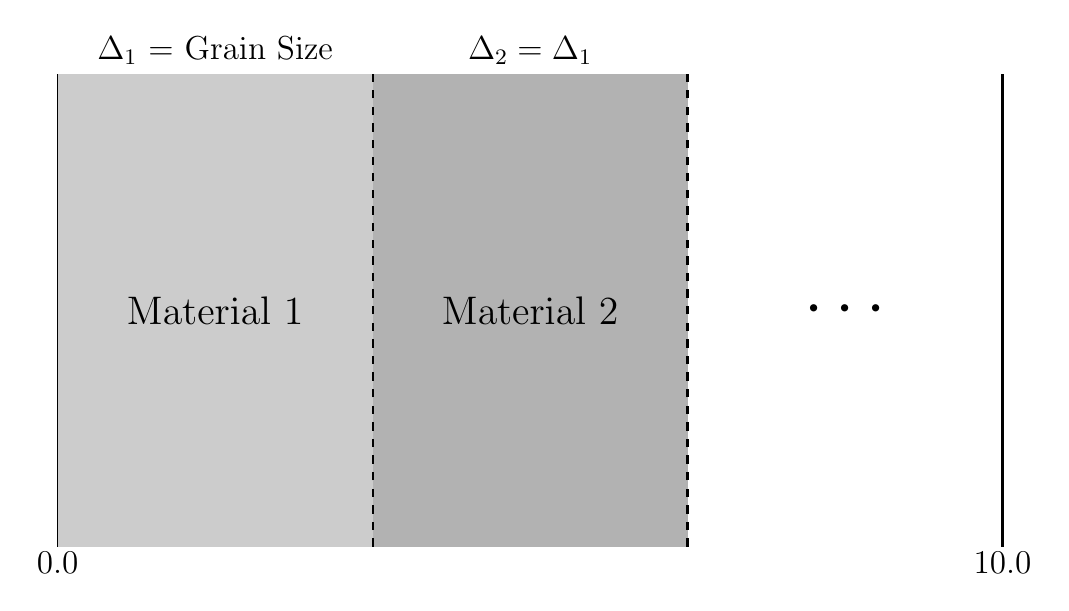
\begin{tikzpicture}
    \begin{scope}[thick,font=\scriptsize]

    \draw [-] (-3,-3) -- (-3,3) {};
    \draw [-] (9,-3) -- (9,3) {};
    
    \draw node at (-3,-3.2) {\large $0.0$};
    \draw node at (9,-3.2) {\large $10.0$};
    
    \fill[fill=black!20] (-3,-3) rectangle (1,3);
    \fill[fill=black!30] (1,-3) rectangle (5,3);
    
    \draw [dashed] (1,-3) -- (1,3) {};
    \draw [dashed] (5,-3) -- (5,3) {};
    
    \draw node at (-1,0) {\Large Material 1};
    \draw node at (3,0) {\Large Material 2};
    \draw node at (7,0) {\Huge{$\cdots$}};
    
    \draw node at (-1,3.3) {\large $\Delta_{1}$ = Grain Size}; 
    \draw node at (3,3.3) {\large $\Delta_{2} = \Delta_{1}$};

    \end{scope}
\end{tikzpicture}
	\caption{Heterogeneous Slab Benchmark Problem Domain \cite{kornreich_timeeigenvalue_2005}}
	\label{fig:HeteroSlabDomain}
\end{figure}

\begin{table}[!htbp]
	\caption{Comparison of RQFP-calculated eigenvalues to various methods for multi-region scattering slab ($M = 500$, $L = 64$, Tolerance = $10^{-12}$)}
	\label{table:RQ_DE_DANT_GFM}
	\begin{subtable}[h]{1.0\textwidth}
	\centering\ra{1.3}
	\begin{tabular}{@{}lccc@{}}\toprule
	& \multicolumn{3}{c}{Alpha-Eigenvalue/Percent Relative Error} \\
	\cmidrule{2-4} Grain Size & RQFP & DANT/PARTISN & \% Relative Error \\
	\midrule
	5 (2 slabs) & $-5.51528 \times 10^{-1}$ & $-5.50813 \times 10^{-1}$ & 0.129782 \\ 
	2.5 (4 slabs) & $-7.03144 \times 10^{-1}$ & $-7.03134 \times 10^{-1}$ & 0.001470 \\ 
	1 (10 slabs) & $-7.48808 \times 10^{-1}$ & $-7.48793 \times 10^{-1}$ & 0.001942 \\ 
	0.5 (20 slabs) & $-7.57221 \times 10^{-1}$ & $-7.57199 \times 10^{-1}$ & 0.002882 \\ 
	0 (homogeneous) & $-7.63513 \times 10^{-1}$ & $-7.63507 \times 10^{-1}$ & 0.000848 \\ 
	\bottomrule
	%\multicolumn{4}{l}{$M = 500$, $L = 64$, Tolerance = $10^{-12}$} \\
	\end{tabular}
	\caption{Comparison of RQFP- and DANT/PARTISN-calculated alpha-eigenvalues}
	\label{AlphaDANT}
	\end{subtable}%
	\vspace{0.25cm}
	\begin{subtable}[h]{1.0\textwidth}
	\centering\ra{1.3}
	\begin{tabular}{@{}lccc@{}}\toprule
	& \multicolumn{3}{c}{Alpha-Eigenvalue/Percent Relative Error} \\
	\cmidrule{2-4} Grain Size & RQFP & GFM & \% Relative Error \\
	\midrule
	5 (2 slabs) & $-5.51528 \times 10^{-1}$ & $-5.50812 \times 10^{-1}$ & 0.129964 \\ 
	2.5 (4 slabs) & $-7.03144 \times 10^{-1}$ & $-7.03133 \times 10^{-1}$ & 0.001612 \\ 
	1 (10 slabs) & $-7.48808 \times 10^{-1}$ & $-7.48792 \times 10^{-1}$ & 0.002075 \\ 
	0.5 (20 slabs) & $-7.57221 \times 10^{-1}$ & $-7.57198 \times 10^{-1}$ & 0.003014 \\ 
	0 (homogeneous) & $-7.63513 \times 10^{-1}$ & $-7.63507 \times 10^{-1}$ & 0.000848 \\ 
	\bottomrule
	%\multicolumn{4}{l}{$M = 500$, $L = 64$, Tolerance = $10^{-12}$} \\
	\end{tabular}
	\caption{Comparison of RQFP- and GFM-calculated alpha-eigenvalues}
	\label{AlphaGFM}
	\end{subtable}%
	\vspace{0.25cm}
	\begin{subtable}[h]{1.0\textwidth}
	\centering\ra{1.3}
	\begin{tabular}{@{}lccc@{}}\toprule
	& \multicolumn{3}{c}{Alpha-Eigenvalue/Percent Relative Error} \\
	\cmidrule{2-4} Grain Size & RQFP & GFM & \% Relative Error \\
	\midrule
	5 (2 slabs) & $-5.51528 \times 10^{-1}$ & $-5.50812 \times 10^{-1}$ & 0.129964 \\ 
	2.5 (4 slabs) & $-7.03144 \times 10^{-1}$ & $-7.03133 \times 10^{-1}$ & 0.001612 \\ 
	1 (10 slabs) & $-7.48808 \times 10^{-1}$ & $-7.48792 \times 10^{-1}$ & 0.002075 \\ 
	0.5 (20 slabs) & $-7.57221 \times 10^{-1}$ & $-7.57198 \times 10^{-1}$ & 0.003014 \\ 
	0 (homogeneous) & $-7.63513 \times 10^{-1}$ & $-7.63507 \times 10^{-1}$ & 0.000848 \\ 
	\bottomrule
	%\multicolumn{4}{l}{$M = 500$, $L = 64$, Tolerance = $10^{-12}$} \\
	\end{tabular}
	\caption{Comparison of RQFP- and DE-calculated alpha-eigenvalues}
	\label{AlphaDE}
	\end{subtable}
\end{table}

%\begin{table*}
%\centering\ra{1.3}
%\caption{Comparison of RQFP- and DANT/PARTISN-calculated alpha-eigenvalues for a multi-region scattering slab}
%\label{AlphaDANT}
%\begin{tabular}{@{}lccc@{}}\toprule
%& \multicolumn{3}{c}{Alpha-Eigenvalue/Percent Relative Error} \\
%\cmidrule{2-4} Grain Size & RQFP & DANT/PARTISN & \% Relative Error \\
%\midrule
%5 (2 slabs) & $-5.51528 \times 10^{-1}$ & $-5.50813 \times 10^{-1}$ & 0.129782 \\ 
%2.5 (4 slabs) & $-7.03144 \times 10^{-1}$ & $-7.03134 \times 10^{-1}$ & 0.001470 \\ 
%1 (10 slabs) & $-7.48808 \times 10^{-1}$ & $-7.48793 \times 10^{-1}$ & 0.001942 \\ 
%0.5 (20 slabs) & $-7.57221 \times 10^{-1}$ & $-7.57199 \times 10^{-1}$ & 0.002882 \\ 
%0 (homogeneous) & $-7.63513 \times 10^{-1}$ & $-7.63507 \times 10^{-1}$ & 0.000848 \\ 
%\bottomrule
%\multicolumn{4}{l}{$M = 500$, $L = 64$, Tolerance = $10^{-12}$} \\
%\end{tabular}
%\end{table*}
%
%\begin{table*}
%\centering\ra{1.3}
%\caption{Comparison of RQFP- and GFM-calculated alpha-eigenvalues for a multi-region scattering slab}
%\label{AlphaGFM}
%\begin{tabular}{@{}lccc@{}}\toprule
%& \multicolumn{3}{c}{Alpha-Eigenvalue/Percent Relative Error} \\
%\cmidrule{2-4} Grain Size & RQFP & GFM & \% Relative Error \\
%\midrule
%5 (2 slabs) & $-5.51528 \times 10^{-1}$ & $-5.50812 \times 10^{-1}$ & 0.129964 \\ 
%2.5 (4 slabs) & $-7.03144 \times 10^{-1}$ & $-7.03133 \times 10^{-1}$ & 0.001612 \\ 
%1 (10 slabs) & $-7.48808 \times 10^{-1}$ & $-7.48792 \times 10^{-1}$ & 0.002075 \\ 
%0.5 (20 slabs) & $-7.57221 \times 10^{-1}$ & $-7.57198 \times 10^{-1}$ & 0.003014 \\ 
%0 (homogeneous) & $-7.63513 \times 10^{-1}$ & $-7.63507 \times 10^{-1}$ & 0.000848 \\ 
%\bottomrule
%\multicolumn{4}{l}{$M = 500$, $L = 64$, Tolerance = $10^{-12}$} \\
%\end{tabular}
%\end{table*}
%
%\begin{table*}
%\centering\ra{1.3}
%\caption{Comparison of RQFP- and DE-calculated alpha-eigenvalues for a multi-region scattering slab}
%\label{AlphaDE}
%\begin{tabular}{@{}lccc@{}}\toprule
%& \multicolumn{3}{c}{Alpha-Eigenvalue/Percent Relative Error} \\
%\cmidrule{2-4} Grain Size & RQFP & DE & \% Relative Error \\
%\midrule
%5 (2 slabs) & $-5.51528 \times 10^{-1}$ & $-5.51429 \times 10^{-1}$ & 0.017928 \\ 
%2.5 (4 slabs)  & $-7.03144 \times 10^{-1}$ & $-7.03578 \times 10^{-1}$ & 0.061637 \\ 
%1 (10 slabs) & $-7.48808 \times 10^{-1}$ & $-7.49672 \times 10^{-1}$ & 0.115312 \\ 
%0.5 (20 slabs) & $-7.57221 \times 10^{-1}$ & $-7.58893 \times 10^{-1}$ & 0.220345 \\ 
%0 (homogeneous) & $-7.63513 \times 10^{-1}$ & $-7.63640 \times 10^{-1}$ & 0.016569 \\ 
%\bottomrule
%\multicolumn{4}{l}{$M = 500$, $L = 64$, Tolerance = $10^{-12}$} \\
%\end{tabular}
%\end{table*}
%
\clearpage

\begin{figure}[!htbp]
	\centering
	\resizebox{0.50\textwidth}{!}{
	\begin{filecontents}{TwoGrain.dat}
x y
0	0.342598000000000
0.500000000000000	0.661696200000000
1.00000000000000	0.914822200000000
1.50000000000000	1.12357700000000
2.00000000000000	1.28413600000000
2.50000000000000	1.39131100000000
3.00000000000000	1.44114600000000
3.50000000000000	1.43155100000000
4.00000000000000	1.36228800000000
4.50000000000000	1.23392300000000
5.00000000000000	1.03445600000000
5.50000000000000	0.835142700000000
6.00000000000000	0.687373800000000
6.50000000000000	0.565772400000000
7.00000000000000	0.463404800000000
7.50000000000000	0.376043900000000
8.00000000000000	0.300536900000000
8.50000000000000	0.234282500000000
9.00000000000000	0.174918500000000
9.50000000000000	0.119789800000000
10	0.0619270900000000
\end{filecontents}

\begin{filecontents}{FourGrain.dat}
x y
0	0.235983600000000
0.500000000000000	0.452301400000000
1.00000000000000	0.617525800000000
1.50000000000000	0.744468000000000
2.00000000000000	0.827526300000000
2.50000000000000	0.847704800000000
3.00000000000000	0.854085000000000
3.50000000000000	0.897244800000000
4.00000000000000	0.963845700000000
4.50000000000000	1.05653300000000
5.00000000000000	1.19968600000000
5.50000000000000	1.32743900000000
6.00000000000000	1.36058700000000
6.50000000000000	1.31752100000000
7.00000000000000	1.20114300000000
7.50000000000000	1.00180800000000
8.00000000000000	0.791621400000000
8.50000000000000	0.622066000000000
9.00000000000000	0.468875900000000
9.50000000000000	0.323710200000000
10	0.168253100000000
\end{filecontents}

\begin{filecontents}{TenGrain.dat}
x y
0	0.218797800000000
0.500000000000000	0.416000600000000
1.00000000000000	0.552000300000000
1.50000000000000	0.672929800000000
2.00000000000000	0.833959100000000
2.50000000000000	0.980485000000000
3.00000000000000	1.03404600000000
3.50000000000000	1.06851200000000
4.00000000000000	1.16887600000000
4.50000000000000	1.24878300000000
5.00000000000000	1.21059700000000
5.50000000000000	1.15092000000000
6.00000000000000	1.16227100000000
6.50000000000000	1.15263500000000
7.00000000000000	1.03395400000000
7.50000000000000	0.897428100000000
8.00000000000000	0.816033400000000
8.50000000000000	0.718689200000000
9.00000000000000	0.552002800000000
9.50000000000000	0.372467500000000
10	0.192713400000000
\end{filecontents}

\begin{filecontents}{TwentyGrain.dat}
x y
0	0.212543500000000
0.500000000000000	0.397013300000000
1.00000000000000	0.557195300000000
1.50000000000000	0.698658000000000
2.00000000000000	0.829517400000000
2.50000000000000	0.940938200000000
3.00000000000000	1.03747300000000
3.50000000000000	1.11214000000000
4.00000000000000	1.16784100000000
4.50000000000000	1.20049700000000
5.00000000000000	1.21136500000000
5.50000000000000	1.19964600000000
6.00000000000000	1.16489100000000
6.50000000000000	1.10964800000000
7.00000000000000	1.03178700000000
7.50000000000000	0.936984800000000
8.00000000000000	0.821495800000000
8.50000000000000	0.693513300000000
9.00000000000000	0.547314300000000
9.50000000000000	0.390898700000000
10	0.198835500000000
\end{filecontents}

\begin{tikzpicture}
\begin{axis}[
        legend style={at={(0.4,0.05)}, anchor = south},
	xlabel=$x$ (MFP),
	ylabel=Scalar Flux $\phi(x)$
]
\addplot[color=red,mark=*] table {TwoGrain.dat};
\addlegendentry{$\Delta = 5$}
\addplot[color=blue,mark=*] table {FourGrain.dat};
\addlegendentry{$\Delta = 2.5$}
\addplot[color=green,mark=*] table {TenGrain.dat};
\addlegendentry{$\Delta = 1$}
\addplot[color=pink,mark=*] table {TwentyGrain.dat};
\addlegendentry{$\Delta = 0.5$}
\end{axis}
\end{tikzpicture}
	}
	\caption{Scalar Flux Results for Alternating Slabs Grain Size Problems}
	\label{fig:GrainScalarFlux}
\end{figure}

\textbf{Problem 6.1.3.2-Multiplying Two Region Heterogeneous Slab}: For a supercritical two-region medium (Figure~\ref{fig:HeteroSlabMult}) consisting of two materials with cross sections given in Table~\ref{table:BetzlerHeteroMult}, the calculated alpha-eigenvalue and scalar flux were compared to the Green's Function Method. The calculated alpha-eigenvalue $\alpha = 0.142473$ s$^{-1}$ agreed with the GFM eigenvalue. The alpha-eigenvalue RQFP method required 48 iterations to converge the problems to a tolerance of $10^{-12}$. The critical search method required 22076 iterations, requiring multiple bracketing attempts. The multiple bracketing attempts were required since the system was close to critical. To verify the correctness of the RQFP alpha-eigenvalue scalar flux, the scalar flux was compared to the GFM scalar flux. The fluxes were found to be in agreement within tolerance (Figure~\ref{fig:TwoRegionMultiply}).

The $k$-effective eigenvalue of the supercritical two-region medium was found to be $1.28656$. The RQFP method was found to require 46 transport sweeps to converge to a tolerance of $10^{-12}$. The power method with fission norm update required 36 transport sweeps.

\begin{figure}[!htbp]
	\centering
	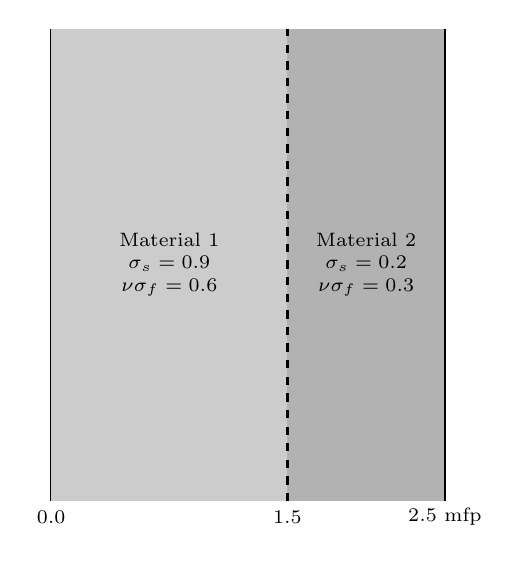
\begin{tikzpicture}[text centered]
    \begin{scope}[thick,font=\scriptsize]

    \draw [-] (-2.5,-3) -- (-2.5,3) {};
    \draw [-] (0.5,-3) -- (0.5,3) {};
    
    \draw node at (-2.5,-3.2) {$0.0$};
    \draw node at (2.5,-3.2) {$2.5$ mfp};
        \draw node at (0.5,-3.2) {$1.5$};
    
    \fill[fill=black!20] (-2.5,-3) rectangle (0.5,3);
    \fill[fill=black!30] (0.5,-3) rectangle (2.5,3);
    
    \draw [dashed] (0.5,-3) -- (0.5,3) {};
    \draw (2.5,-3) -- (2.5,3) {};
    
    \draw node [align=center] at (-1.0,0) {Material 1 \\ $\sigma_{s} = 0.9$ \\ $\nu \sigma_{f} = 0.6$};
    \draw node [align=center] at (1.5,0) {Material 2 \\ $\sigma_{s} = 0.2$ \\ $\nu \sigma_{f} = 0.3$};


    \end{scope}
\end{tikzpicture}
	\caption{Heterogeneous Multiplying Slab Benchmark Problem Domain \cite{kornreich_greens_1997}}
	\label{fig:HeteroSlabMult}
\end{figure}

\begin{figure}[!htbp]
	\centering
	\resizebox{0.5\textwidth}{!}{
	\begin{filecontents}{AlphaRQFP.dat}
x y
0.00E+00 1
1.50E-01 1.447247465
3.00E-01 1.755560563
4.50E-01 1.980425738
6.00E-01 2.125210861
7.50E-01 2.188765251
9.00E-01 2.169994135
1.05E+00 2.068765518
1.20E+00 1.885253322
1.35E+00 1.616038124
1.50E+00 1.208241837
1.60E+00 0.942444665
1.70E+00 0.777235239
1.80E+00 0.651820797
1.90E+00 0.551556358
2.00E+00 0.469075409
2.10E+00 0.399845272
2.20E+00 0.340724486
2.30E+00 0.289282031
2.40E+00 0.24323767
2.50E+00 0.198355012
\end{filecontents}

\begin{filecontents}{AlphaGFM.dat}
x    y
0    1
0.15 1.4573313
0.30 1.7677868
0.45 1.9942160
0.60 2.1400088
0.75 2.2040045
0.90 2.1851026
1.05 2.0831691
1.20 1.8983807
1.35 1.6272924
1.50 1.2166341
1.60 0.94899798
1.70 0.78264174
1.80 0.65635543
1.90 0.55539366
2.00 0.47233885
2.10 0.40262710
2.20 0.34309503
2.30 0.29129485
2.40 0.24493022
2.50 0.19900451
\end{filecontents}

\begin{tikzpicture}
\begin{axis}[
	xlabel=$x$ (MFP),
	ylabel=Scalar Flux $\phi(x)$
]
\addplot[color=red,mark=*] table {AlphaRQFP.dat};
\addlegendentry{RQFP}
\addplot[color=blue,mark=o] table {AlphaGFM.dat};
\addlegendentry{GFM}
\end{axis}
\end{tikzpicture}
	}
	\caption{Alpha-Eigenvalue Scalar Flux Results for Two-Region Multiplying Slab}
	\label{fig:TwoRegionMultiply}
\end{figure}

\clearpage
\textbf{Problem 6.1.3.3-Multiplying Five Region Fuel-Pin}:

A five region fuel-pin-like domain was modeled ($M=1000$ and $L=64$) and the alpha-eigenvalues compared to GFM for four cases. For case one and two, the fuel-pin domain consisted of five regions as seen in Figure~\ref{fig:FiveRegionProblem}, fuel, moderator, absorber, moderator, and fuel, with cross sections given in Table~\ref{table:BetzlerFive}. The leftmost fuel pin had a one mean free path width. For case one and two, the fuel fission cross section was set to $\nu \sigma_{f} = 0.3$ or $\nu \sigma_{f} = 0.7$. The alpha-eigenvalues were $\alpha = -0.3197041$ s$^{-1}$ and $\alpha = -0.0062120$ s$^{-1}$ for the $\nu \sigma_{f} = 0.3$ and $\nu \sigma_{f} = 0.7$ cases, respectively. The RQFP method eigenvalues matched the GFM-calculated alpha-eigenvalues within tolerance. Convergence of the $\nu \sigma_{f} = 0.3$ and $\nu \sigma_{f} = 0.7$ cases for the RQFP method required 30 and 27 transport sweeps, respectively. The scalar fluxes for both cases matched GFM within tolerance and are seen in Figure~\ref{fig:FiveRegionMultiply}. For cases three and four, the leftmost fuel pin width was set to 1.1. The alpha-eigenvalues for $\nu \sigma_{f} = 0.3$ and $\nu \sigma_{f} = 0.7$ were found to be -0.2932897 s$^{-1}$ and 0.0375543 s$^{-1}$, respectively. The RQFP method eigenvalues matched the GFM-calculated alpha-eigenvalues within tolerance (Table~\ref{table:FiveRegionCases}). For the supercritical case, the alpha-eigenvalue RQFP required 502 sweeps as compared to 13099 sweeps for the critical search method.

For leftmost fuel pin width of one mean free path, the $k$-effective eigenvalue of the five region fuel-pin-like was determined to be $0.42428$ and $0.98998$ for the $\nu \sigma_{f} = 0.3$ and $\nu \sigma_{f} = 0.7$ cases, respectively. For the $\nu \sigma_{f} = 0.3$ fuel pin, the RQFP method required 29 transport sweeps while the power method with fission norm update required 22 transport sweeps. For the $\nu \sigma_{f} = 0.7$ fuel pin, the RQFP method required 28 transport sweeps while the power method with fission norm update required 21 transport sweeps. For leftmost fuel pin width of 1.1 mean free paths, the $k$-effective was determined to be $0.45554$ and $1.06316$, respectively, for  $\nu \sigma_{f} = 0.3$ and $\nu \sigma_{f} = 0.7$. For the $\nu \sigma_{f} = 0.3$ fuel pin, the RQFP method required 514 transport sweeps while the power method with fission norm update required 355 transport sweeps. For the $\nu \sigma_{f} = 0.7$ fuel pin, the RQFP method required 513 transport sweeps while the power method with fission norm update required 355 transport sweeps.

\begin{figure}[h]
	\centering
	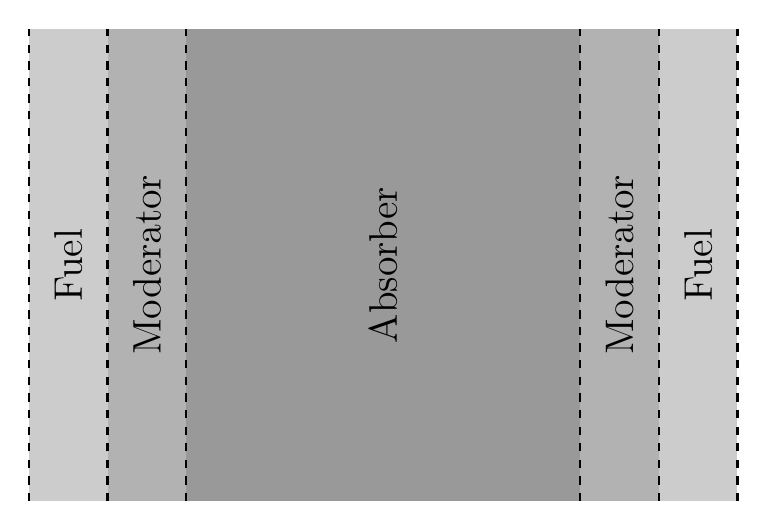
\begin{tikzpicture}
    \begin{scope}[thick,font=\scriptsize]
    
    \fill[fill=black!20] (-4.5,-3) rectangle (-3.5,3);
    \fill[fill=black!30] (-3.5,-3) rectangle (-2.5,3);
    \fill[fill=black!40] (-2.5,-3) rectangle (2.5,3);
        \fill[fill=black!30] (2.5,-3) rectangle (3.5,3);
            \fill[fill=black!20] (3.5,-3) rectangle (4.5,3);
    
    \draw [dashed] (-4.5,-3) -- (-4.5,3) {};
    \draw [dashed] (-3.5,-3) -- (-3.5,3) {};
    \draw [dashed] (-2.5,-3) -- (-2.5,3) {};
    \draw [dashed] (2.5,-3) -- (2.5,3) {};
   \draw [dashed] (3.5,-3) -- (3.5,3) {};
   \draw [dashed] (4.5,-3) -- (4.5,3) {};
   
   \draw node at (-4,0) {\Large \rotatebox[origin=c]{90}{Fuel}};
   \draw node at (-3,0) {\Large \rotatebox[origin=c]{90}{Moderator}};  
   \draw node at (-0,0) {\Large \rotatebox[origin=c]{90}{Absorber}};
   \draw node at (3,0) {\Large \rotatebox[origin=c]{90}{Moderator}};
   \draw node at (4,0) {\Large \rotatebox[origin=c]{90}{Fuel}};  

    \end{scope}
\end{tikzpicture}
	\caption{Five Region Heterogeneous Slab Benchmark Problem Domain \cite{kornreich_timeeigenvalue_2005}}
	\label{fig:FiveRegionProblem}
\end{figure}

\begin{table*}[!htbp]
\centering\ra{1.3}
\caption{Comparison of RQFP- and GFM-calculated alpha-eigenvalues for Multiplying Five-region Fuel-pin}
\label{table:FiveRegionCases}
\begin{tabular}{@{}ccccc@{}}\toprule
& & \multicolumn{3}{c}{Alpha-Eigenvalue/Percent Relative Error} \\
\cmidrule{3-5} $\Delta$ & $\nu \sigma_{f}$ & RQFP & GFM & \% Relative Error \\
\midrule
%$\Delta$\\
1 & 0.3 & $-3.197041 \times 10^{-1}$ & $-3.196537 \times 10^{-2}$ & $1.58 \times 10^{-2}$ \\ 
1 & 0.7 & $-6.212026 \times 10^{-3}$ & $-6.156369 \times 10^{-3}$ & $9.041 \times 10^{-1}$ \\ 
1.1 & 0.3 & $-2.932897 \times 10^{-1}$ & $-2.93247 \times 10^{-1}$ & $1.46 \times 10 ^{-2}$ \\ 
1.1 & 0.7 & $3.75543 \times 10^{-2}$ & $3.759991 \times 10^{-2}$ & $1.213 \times 10^{-1}$ \\ 
\bottomrule
\multicolumn{5}{l}{$M = 1000$, $L = 64$, Tolerance = $10^{-12}$} \\
\end{tabular}
\end{table*}

\begin{figure}[!htbp]
	\centering
	\resizebox{0.5\textwidth}{!}{
	\begin{filecontents}{Alpha03.dat}
x y
-4.500000e+00 4.988790e-01
-4.250000e+00 7.311603e-01
-4.000000e+00 8.484920e-01
-3.750000e+00 8.770258e-01
-3.500000e+00 7.985426e-01
-3.250000e+00 6.820846e-01
-3.000000e+00 5.835900e-01
-2.750000e+00 4.767421e-01
-2.500000e+00 3.391279e-01
-2.250000e+00 2.279149e-01
-2.000000e+00 1.689942e-01
-1.750000e+00 1.297957e-01
-1.500000e+00 1.022940e-01
-1.250000e+00 8.259903e-02
-1.000000e+00 6.848630e-02
-7.500000e-01 5.858579e-02
-5.000000e-01 5.203239e-02
-2.500000e-01 4.829319e-02
0.000000e+00 4.707760e-02
2.500000e-01 4.829319e-02
5.000000e-01 5.203239e-02
7.500000e-01 5.858579e-02
1.000000e+00 6.848630e-02
1.250000e+00 8.259903e-02
1.500000e+00 1.022940e-01
1.750000e+00 1.297957e-01
2.000000e+00 1.689942e-01
2.250000e+00 2.279149e-01
2.500000e+00 3.391279e-01
2.750000e+00 4.767421e-01
3.000000e+00 5.835900e-01
3.250000e+00 6.820846e-01
3.500000e+00 7.985426e-01
3.750000e+00 8.770258e-01
4.000000e+00 8.484920e-01
4.250000e+00 7.311603e-01
4.500000e+00 4.988790e-01
\end{filecontents}

\begin{filecontents}{Alpha07.dat}
-4.500000e+00 6.530922e-01
 -4.250000e+00 1.042446e+00
 -4.000000e+00 1.205673e+00
 -3.750000e+00 1.177297e+00
 -3.500000e+00 9.175721e-01
 -3.250000e+00 6.420169e-01
 -3.000000e+00 4.797641e-01
 -2.750000e+00 3.521589e-01
 -2.500000e+00 2.296407e-01
 -2.250000e+00 1.415589e-01
 -2.000000e+00 9.587206e-02
 -1.750000e+00 6.705560e-02
 -1.500000e+00 4.798165e-02
 -1.250000e+00 3.508555e-02
 -1.000000e+00 2.632529e-02
 -7.500000e-01 2.045971e-02
 -5.000000e-01 1.671996e-02
 -2.500000e-01 1.464154e-02
 0.000000e+00 1.397496e-02
 2.500000e-01 1.464154e-02
 5.000000e-01 1.671996e-02
 7.500000e-01 2.045971e-02
 1.000000e+00 2.632529e-02
 1.250000e+00 3.508555e-02
 1.500000e+00 4.798165e-02
 1.750000e+00 6.705560e-02
 2.000000e+00 9.587206e-02
 2.250000e+00 1.415589e-01
 2.500000e+00 2.296407e-01
 2.750000e+00 3.521589e-01
 3.000000e+00 4.797641e-01
 3.250000e+00 6.420169e-01
 3.500000e+00 9.175721e-01
 3.750000e+00 1.177297e+00
 4.000000e+00 1.205673e+00
 4.250000e+00 1.042446e+00
 4.500000e+00 6.530922e-01
\end{filecontents}

\begin{tikzpicture}
\begin{axis}[
	xlabel=$x$ (MFP),
	ylabel=Scalar Flux $\phi(x)$
]
\addplot[color=red,mark=*] table {Alpha03.dat};
\addlegendentry{$\nu \sigma_{f} = 0.3$}
\addplot[color=blue,mark=*] table {Alpha07.dat};
\addlegendentry{$\nu \sigma_{f} = 0.7$}
\end{axis}
\end{tikzpicture}
	}
	\caption{Case One and Two Scalar Flux Results for Five-Region Multiplying Slab-Two Cases}
	\label{fig:FiveRegionMultiply}
\end{figure}

\section{Multigroup Verification for Slab Geometry}

\clearpage
\section{One-Speed Verification for Spherical Geometry}

In certain circumstances, alpha-eigenvalue results for slab geometry also apply to spherical geometry problems. This slab-sphere equivalence holds for isotropically scattering heterogeneous media where the total cross section is equal for all regions \cite{davison1957neutron}. More generally, a convenient property of spherically symmetric systems is that if the mean free path in the system is independent of position and scattering is isotropic, then the determination of the spherically symmetric neutron distribution of these systems is reduced to the determination of these distributions in certain systems with plane symmetries. Thus, for all homogeneous slab and symmetric heterogeneous slab systems where each region has the same total cross section, it follows that there exists a spherical equivalent for the problems studied in the previous sections. Specifically, it can be shown that the second eigenvalue of a slab system is identical to the fundamental eigenvalue for the equivalent sphere. In this section, we examine the performance of the RQFP method for one-dimensional spherical problems which are equivalent to the slab problems from before. We verify the correctness of the method for this subset of problems and compare its performance to the critical search and power methods.

\subsection{Non-Multiplying Homogeneous Spheres}

\begin{table*}[t]
\centering\ra{1.3}
\caption{Comparison of RQFP- and GFM-calculated alpha-eigenvalues for a homogeneous scattering sphere}
\label{table:CompHomogScattSphere}
\begin{tabular}{@{}cccc@{}}\toprule
& \multicolumn{3}{c}{Alpha-Eigenvalue/Percent Relative Error} \\
\cmidrule{2-4} $\Delta$ & RQFP & GFM & \% Relative Error \\
\midrule
5 & $-3.41177 \times 10^{-1}$ & $-3.41216 \times 10^{-1}$ & 0.0114 \\ 
10 & $-1.02973 \times 10^{-1}$ & $-1.02978 \times 10^{-1}$ & 0.0049 \\ 
20 & $-2.88443 \times 10^{-2}$ & $-2.88447 \times 10^{-2}$ & 0.0014 \\ 
25 & $-1.89226 \times 10^{-2}$ & $-1.89228 \times 10^{-2}$ & 0.0011 \\ 
\bottomrule
\multicolumn{4}{l}{$M = 500$, $L = 64$, Tolerance = $10^{-12}$} \\
\end{tabular}
\end{table*}

\subsection{Multiplying Homogeneous Spheres}

\begin{table*}[h]
\centering\ra{1.3}
\caption{Comparison of RQFP- and GFM-calculated alpha-eigenvalues for a homogeneous scattering multiplying sphere}
\label{table:CompHomogMultSphere}
\begin{tabular}{@{}cccc@{}}\toprule
& \multicolumn{3}{c}{Alpha-Eigenvalue/Percent Relative Error} \\
\cmidrule{2-4} $\Delta$ & RQFP & GFM & \% Relative Error \\
\midrule
3 & $-5.68218 \times 10^{-1}$ & $-5.6833 \times 10^{-1}$ & 0.0197 \\ 
4 & $-3.00486 \times 10^{-1}$ & $-3.0054 \times 10^{-1}$ & 0.0180 \\ 
5 & $ -1.60321 \times 10^{-1}$ & $-1.6035 \times 10^{-1}$ & 0.0181 \\ 
6 & $ -7.72739 \times 10^{-2}$ & $-7.7292 \times 10^{-2}$ & 0.0234 \\ 
7 & $-2.38450 \times 10^{-2}$ & $-2.3857 \times 10^{-2}$ & 0.0503 \\ 
8 & $1.26235 \times 10^{-2}$ & $1.2616 \times 10^{-2}$ & 0.0594 \\ 
9 & $ 3.86541 \times 10^{-2}$ & $3.8649 \times 10^{-2}$ & 0.0132 \\ 
10 & $5.78980 \times 10^{-2}$ & $5.7894 \times 10^{-2}$ & 0.0069 \\ 
15 & $1.06258 \times 10^{-1}$ & $1.0626 \times 10^{-1}$ & 0.0019 \\ 
20 & $1.24512 \times 10^{-1}$ & $1.2451 \times 10^{-1}$ &  0.0016 \\ 
30 & $1.38248 \times 10^{-1}$ & $1.3825 \times 10^{-1}$ &  0.0014 \\ 
40 & $1.43262 \times 10^{-1}$ & $1.4326 \times 10^{-1}$ &  0.0014 \\ 
50 & $1.45638 \times 10^{-1}$ & $1.4564 \times 10^{-1}$ &  0.0014 \\ 
\bottomrule
\multicolumn{4}{l}{$M = 500$, $L = 64$, Tolerance = $10^{-12}$} \\
\end{tabular}
\end{table*}

\begin{table}[!htbp]
	\caption{Transport Sweep Comparisons for Homogeneous Multiplying Spheres}
	\begin{subtable}[h]{1.0\textwidth}
	\centering\ra{1.3}
	\begin{tabular}{@{}cccccc@{}}\toprule
	& \multicolumn{2}{c}{Transport Sweeps} & & \multicolumn{2}{c}{Transport Sweeps} \\
	\cmidrule{2-3} \cmidrule{5-6} $\Delta$ & RQFP & Critical Search \quad &  \Delta & RQFP & Critical Search\\
	\midrule
3 & 46 & * & 10 & 128 & 29645 \\
4 & 46 & * & 15 & 227 & 61303 \\
5 & 52 & * & 20 & 357 & 84353 \\
6 & 67 & * & 30 & 707 & 100433 \\
7 & 81 & * & 40 & 1176 & 99135 \\
8 & 96 & 10865 & 50 & 1761 & 97037 \\
9 & 111 & 21555 & & & \\ 
	\bottomrule
	\multicolumn{6}{l}{*Did Not Converge} \\
	\end{tabular}
	\caption{Alpha-Eigenvalue: Comparison of RQFP and Critical Search Sweeps}
	\label{table:CompMultSweepsSphere}
	\end{subtable}%
	\vspace{0.25cm}
	\begin{subtable}[h]{1.0\textwidth}
	\centering\ra{1.3}
	\begin{tabular}{@{}cccccc@{}}\toprule
	& \multicolumn{2}{c}{Transport Sweeps} & & \multicolumn{2}{c}{Transport Sweeps} \\
	\cmidrule{2-3} \cmidrule{5-6} $\Delta$ & RQFP & Power Method \quad &  \Delta & RQFP & Power Method\\
	\midrule
3 & 49 & 43 & 10 & 127 & 62 \\ 
4 & 57 & 47 & 15 & 214 & 79 \\
5 & 66 & 49 & 20 & 329 & 103 \\
6 & 76 & 52 & 30 & 636 & 167 \\ 
7 & 87 & 54 & 40 & 1049 & 253 \\ 
8 & 99 & 56 & 50 & 1562 & 360 \\ 
9 & 113 & 59 &  &  &  \\ 
	\bottomrule
	\multicolumn{6}{l}{$M = 500$, $L = 64$, Tolerance = $10^{-12}$} \\
	\end{tabular}
	\caption{$k$-Effective: Comparison of RQFP and Power Method Transport Sweeps}
	\label{table:CompMultSweepsKSphere}
	\end{subtable}
\end{table}

%\begin{table*}[t]
%\centering\ra{1.3}
%\caption{Alpha-Eigenvalue: Comparison of RQFP and Critical Search Sweeps for Homogeneous Multiplying Spheres}
%\label{table:CompMultSweepSpheres}
%\begin{tabular}{@{}cccccc@{}}\toprule
%& \multicolumn{2}{c}{Transport Sweeps} & & \multicolumn{2}{c}{Transport Sweeps} \\
%\cmidrule{2-3} \cmidrule{5-6} $\Delta$ & RQFP & Critical Search \quad &  \Delta & RQFP & Critical Search\\
%\midrule
%%$\Delta$\\
%%8 & 98 & 10865 & 20 & 364 & 84353\\ 
%%9 & 113 & 21555 & 30 & 722 & 100433 \\
%%10 & 130 & 29645 & 40 & 1201 & 99135 \\
%%15 & 232 & 61303 & 50 & 1799 & 97037 \\
%3 & x & * & 10 & 130 & 29645 \\
%4 & x & * & 15 & 232 & 61303 \\
%5 & x & * & 20 & 364 & 84353 \\
%6 & x & * & 30 & 722 & 100433 \\
%7 & x & * & 40 & 1201 & 99135 \\
%8 & 98 & 10865 & 50 & 1799 & 97037 \\
%9 & 113 & 21555 & & & \\ 
%\bottomrule
%\multicolumn{6}{l}{$M = 500$, $L = 64$, Tolerance = $10^{-12}$} \\
%\end{tabular}
%\end{table*}
%
%\begin{table*}[t]
%\centering\ra{1.3}
%\caption{$k$-Effective Eigenvalue: Comparison of RQFP and Power Method with Fission Norm Sweeps for Homogeneous Multiplying Spheres}
%\label{table:CompMultSweepSpheresK}
%\begin{tabular}{@{}cccccc@{}}\toprule
%& \multicolumn{2}{c}{Transport Sweeps} & & \multicolumn{2}{c}{Transport Sweeps} \\
%\cmidrule{2-3} \cmidrule{5-6} $\Delta$ & RQFP & Power Method \quad &  \Delta & RQFP & Power Method\\
%\midrule
%%$\Delta$\\
%3 & 49 & 43 & 10 & 127 & 62 \\ 
%4 & 57 & 47 & 15 & 214 & 79 \\
%5 & 66 & 49 & 20 & 329 & 103 \\
%6 & 76 & 52 & 30 & 636 & 167 \\ 
%7 & 87 & 54 & 40 & 1049 & 253 \\ 
%8 & 99 & 56 & 50 & 1562 & 360 \\ 
%9 & 113 & 59 &  &  &  \\ 
%\bottomrule
%\multicolumn{6}{l}{$M = 500$, $L = 64$, Tolerance = $10^{-12}$} \\
%\end{tabular}
%\end{table*}

\begin{figure}[!htbp]
	\centering
	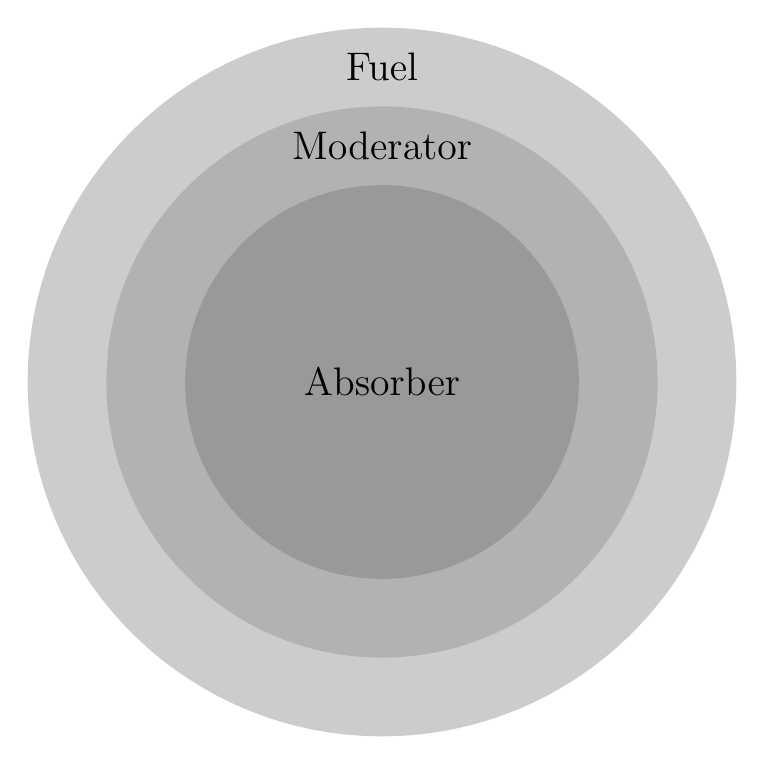
\begin{tikzpicture}
    \begin{scope}[thick,font=\scriptsize]
   
    \fill[fill=black!20] circle (4.5);
    \fill[fill=black!30] circle (3.5);    
    \fill[fill=black!40] circle (2.5);    
    
    \draw node at (0,0) {\Large \rotatebox[origin=c]{0}{Absorber}};
    \draw node at (0,3) {\Large \rotatebox[origin=c]{0}{Moderator}};  
    \draw node at (0,4) {\Large \rotatebox[origin=c]{0}{Fuel}};  
%   \draw node at (-4,0) {\Large \rotatebox[origin=c]{90}{Fuel}};
%   \draw node at (-3,0) {\Large \rotatebox[origin=c]{90}{Moderator}};  
%   \draw node at (-0,0) {\Large \rotatebox[origin=c]{90}{Absorber}};
%   \draw node at (3,0) {\Large \rotatebox[origin=c]{90}{Moderator}};
%   \draw node at (4,0) {\Large \rotatebox[origin=c]{90}{Fuel}};  

    \end{scope}
\end{tikzpicture}
	\caption{Five Region Fuel Pin Spherical Equivalent \cite{kornreich_timeeigenvalue_2005}}
	\label{fig:FiveRegionSphereProblem}
\end{figure}

\begin{table*}[!htbp]
\centering\ra{1.3}
\caption{Comparison of RQFP- and GFM-calculated alpha-eigenvalues for a three region multiplying sphere}
\label{table:FiveRegionCasesSphere}
\begin{tabular}{@{}ccccc@{}}\toprule
& & \multicolumn{3}{c}{Alpha-Eigenvalue/Percent Relative Error} \\
\cmidrule{3-5} $\Delta$ & $\nu \sigma_{f}$ & RQFP & GFM & \% Relative Error \\
\midrule
%$\Delta$\\
1 & 0.3 & $-3.213384 \times 10^{-1}$ & $-3.229855 \times 10^{-1}$ & $5.10 \times 10^{-1}$ \\ 
1 & 0.7 & $-6.300281 \times 10^{-3}$ & $-6.440766 \times 10^{-3}$ & $2.18$ \\ 
\bottomrule
\multicolumn{5}{l}{$M = 1000$, $L = 64$, Tolerance = $10^{-12}$} \\
\end{tabular}
\end{table*}

\subsection{Multiplying Homogeneous Spheres with Anisotropic Scattering}

\begin{table}[!htbp]
	\caption{Uranium-Heavy Water Cross Sections with Anisotropic Scattering for Critical Sphere Problems (cm$^{-1}$) \cite{sood2003analytical}}
	\label{table:SoodUD2OAniso}
	\centering\ra{1.3}
    \begin{tabular}{*6c}
        \toprule
	Cross Section Set & $\sigma$ & $\nu \sigma_{f}$ & $\sigma_{s0}$  & $\sigma_{s1}$ & $v$ [cm/s] \\ 
        \midrule
	U-D$_{2}$O (a)  & 0.54628 & 0.098788237268 & 0.464338 & 0.056312624 & 1 \\
	U-D$_{2}$O (b)  & 0.54628 & 0.100574846008 & 0.464338 & 0.112982569 & 1 \\
	U-D$_{2}$O (c)  & 0.54628 & 0.0926709392 & 0.464338 & -0.27850447 & 1 \\
        \bottomrule
    \end{tabular}
\end{table}

\begin{table}[!htbp]
	\caption{Calculated Eigenvalues and Transport Sweep Comparisons for Critical Sphere Problems with Anisotropic Scattering in \cite{sood2003analytical}}
	\label{table:AnisoSphere}
	\begin{subtable}[h]{1.0\textwidth}
	\centering\ra{1.3}
	\begin{tabular}{@{}cccc@{}}\toprule
	& & \multicolumn{2}{c}{Transport Sweeps} \\
	\cmidrule{3-4} Cross Section Set & Calculated $\alpha$ [s$^{-1}$] & RQFP & Critical Search\\
	\midrule
	U-D$_{2}$O (a) & $3.165772 \times 10^{-7}$ & 299 & 585 \\
	U-D$_{2}$O (b) & $3.930857 \times 10^{-7}$ & 270 & 541\\
	U-D$_{2}$O (c) & $ -6.613381 \times 10^{-7}$ & 456 & *\\
	\bottomrule
	\multicolumn{4}{l}{*Did Not Converge} \\
	\end{tabular}
	\caption{Alpha-Eigenvalue: Comparison of RQFP and Critical Search Transport Sweeps}
	\label{table:AnisoSphereAlpha}
	\end{subtable}%
	\vspace{0.25cm}
	\begin{subtable}[h]{1.0\textwidth}
	\centering\ra{1.3}
	\begin{tabular}{@{}cccc@{}}\toprule
	& & \multicolumn{2}{c}{Transport Sweeps} \\
	\cmidrule{3-4} Cross Section Set & Reference $k_{\text{eff}}$ & RQFP & Power Method \\
	\midrule
	U-D$_{2}$O (a) & 1.000003 & 301 & 118 \\
	U-D$_{2}$O (b) & 1.000003 & 273 & 106 \\
	U-D$_{2}$O (c) & 0.999993 & 456 & 207 \\
	\bottomrule
	\multicolumn{4}{l}{$M = 500$, $L = 64$, Tolerance = $10^{-12}$} \\
	\end{tabular}
	\caption{$k$-Effective: Comparison of RQFP and Power Method Transport Sweeps}
	\label{table:AnisoSpherek}
	\end{subtable}
\end{table}

\section{Multigroup Verification for Spherical Geometry}

\section{Conclusion}

%\begin{table*}
%\centering\ra{1.3}
%\begin{tabular}{@{}rrrr@{}}\toprule
%
%& \multicolumn{3}{c}{$w = 8$} \\
%\cmidrule{2-4} & $t=0$ & $t=1$ & $t=2$ \\
%\midrule$dir=1$\\
%$c$ & 0.0790 & 0.1692 & 0.2945 \\
%$c$ &  -0.8651& 50.0476& 5.9384 \\
%$c$ & 124.2756& -50.9612& -14.2721 \\
%$dir=0$\\
%$c$ & 0.0357& 1.2473& 0.2119 \\
%$c$ & -17.9048& -37.1111& 8.8591 \\
%$c$ & 105.5518& 232.1160& -94.7351\\
%\bottomrule
%\end{tabular}
%\caption{Caption}
%\end{table*}